\documentclass{article}
\usepackage[utf8]{inputenc}

\title{Manual de usuario}
\author{Matriz 8x8 de leds}
\date{Abril 2021}

\usepackage{natbib}
\usepackage{graphicx}

\begin{document}

\maketitle

\section{Introducción}
Debido al aumento de la complejidad en las recientes innovaciones en general, es necesario emplear nuevas técnicas que le faciliten al individuo el uso de las herramientas de las que dispone. Un manual de usuario es de los más tradicionales y efectivos métodos que guían a las personas en el correcto uso de un aparato en general. 

Entonces para este proyecto, en donde su uso está orientado a cierta población, es necesario crear una guía que le permita al usuario aprender a usarlo, y que sea una agradable experiencia.

\section{Manual de usuario}
Algo importante que mencionar es que la forma en que el usuario interactúa con el programa y selecciona las opciones que se le presentan es por medio de numeros. Cada numero corresponde a las opciones disponibles. En caso de que ingrese algo que no corresponde a alguna de las opciones se le mostrará un aviso y, automáticamente, el programa vuelve al menú principal. 

\subsection{Abrir el programa}
Una vez haya ingresado al enlace del proyecto en Tinkercad
se abrirá el diseño de 64 leds antes mencionado.
Para hacer que le proyecto empiece a funcionar se debe dar clic en el siguiente botón:

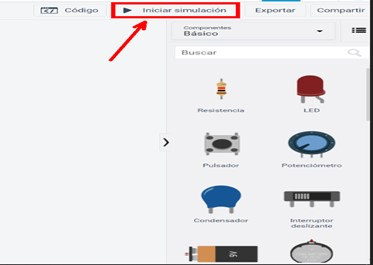
\includegraphics[scale=0.6]{images/IniciarSimulacion.jpg}
\newline

Luego de iniciar la simulación se da clic en el botón “Código”:

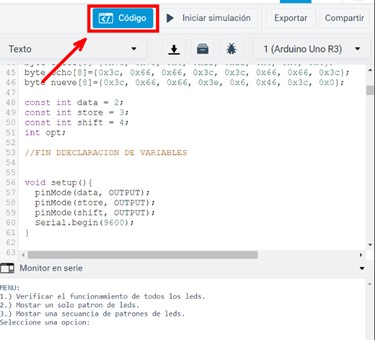
\includegraphics[scale=0.6]{images/Codigo.jpg}
\newline

Posteriormente se dará clic en "Monitor en serie":

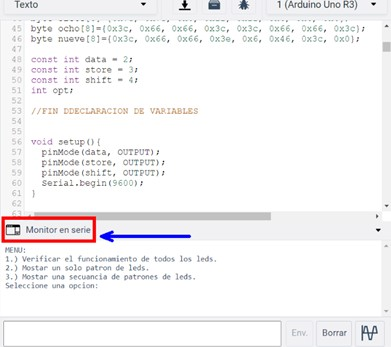
\includegraphics[scale=0.5]{images/MonitorSerial.jpg}
\newline

Una vez hecho los pasos antes mencionados, se muestra un cuadro de menú;

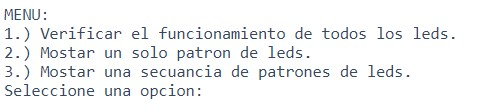
\includegraphics[scale=0.9]{images/Menu.jpg}
\newline

El usuario tiene la posibilidad de escoger cualquiera de las tres opciones mostradas en  la imagen anterior. 

\subsection{Opciones del menú}
Del menú anteriormente mencionado, pueden ocurrir 4 casos:

\begin{enumerate}
    \item 
    Si el usuario ingresa el numero 1 se realizará una prueba de encendido de todos los leds. Todos los leds se encenderán. 
    \item
    En caso de que se ingrese el numero 2, se desplegará el siguiente submenú de opciones:
    
    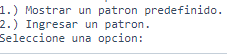
\includegraphics[scale=1]{images/Submenu.png}
    \begin{itemize}
        \item 
        Si en el submenú ingresa la opcion numero 1 se le pedirá que ingrese un caracter cualquiera desde a 'A' hasta la 'Z' o un numero entre '0' o '9'. 
        Una vez ingresado el caracter en la consola serial, presiona ENTER o en el boton 'Enviar', al lado derecho de donde ingresa los datos, para que el programa inicie el proceso de encendido de los leds. 
        El encendido coindidirá con el caracter ingresado.
        \item
        Si el usuario ingresa el numero 2 se mostrará lo siguiente:
        
        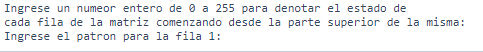
\includegraphics[scale=0.9]{images/SubMenuOpc2.png}
        
        Para poder mostrar un patrón el usuario deberá ingresar el estado de cada fila de la matriz. Serán números que cumplan el rango desde 0 hasta el 255 ya que ambos son los casos extremos: cero para todos apagados, y 255 para todos encendidos. 
        \newline
        
        Esto basados en los números binarios, ya que el 255 en binario seria 11111111 y el 0 seria 00000000. Los leds se encederán según el numero binario, uno (1) para encendido y cero (0) para apagado, leyéndolos de derecha a izquierda. 
        Un ejemplo sería: 
        si el usuario ingresa 60, 66, 165, 129, 165, 153, 66 y 60 se mostrará una carita feliz. Importante tener en cuenta que cada numero corresponde a cada fila, empezado desde donde están las resistencias. 
        \newline
        
        Si el usuario ingresa algo diferente a los numeros 1 o 2, se imprime: "Opción fuera de rango"; y se volverá al menú principal. También, luego de que se muestre el patrón seleccionado, se volverá al menú principal. 
        
    \end{itemize}
    
    \item
    Después, si se ingresa la opción 3, primeramente, el usuario deberá indicar cuantos patrones desea mostrar en la matriz. Luego de esto, se le pide al usuario que ingrese de la siguiente manera el estado de cada fila de cada secuencia de leds (Nuevamente serán números enteros desde el 0 hasta el 255 y con la misma idea)
    
    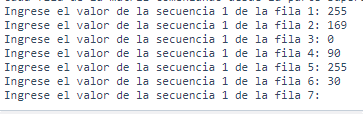
\includegraphics[scale=0.7]{images/MuestraSecuencias.png}
    
    Luego de esto, se le pide al usuario que ingrese cuánto tiempo desea que se muestre cada patrón, para así mostrar los patrones en el tiempo requerido.
    \newline
    Una vez terminado de mostrar cada uno de los patrones, de volverá nuevamente al menú principal. 
    \item
    Si se ingresa un valor diferente a los numero 1, 2 y 3 se mostrará el siguiente aviso: "Opción fuera de rango". Luego, vuelve al menú principal. 
\end{enumerate}

\subsection{Finalizar ejecución del programa}
Terminado el tiempo de ejecución de cada funcionalidad, se volverá a mostrar el menú inicial (Imagen 3) y de nuevo pedirá al usuario un número del menú, que desee ejecutar.
\newline

Una vez terminado la ejecución del programa, se finaliza de la siguiente forma: s da clic en el botón “Detener ejecución” como se muestra en la imagen. 

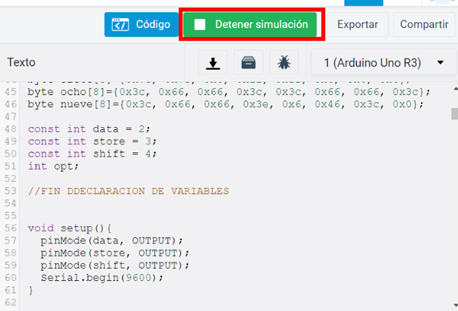
\includegraphics[scale=0.8]{images/Finalizar.png}

\end{document}
